%% start of file `main.tex'.
%% Copyright 2014 Francois Mouton (moutonf@gmail.com).
%
% This template is adapted from the work performed by Xavier Danaux (xdanaux@gmail.com).
% This template further extends the functionality by integrating the moderntimeline package.
% This template also includes custom Biblatex style to print bibliography items with the moderntimeline package.
%
% This work may be distributed and/or modified under the
% conditions of the LaTeX Project Public License version 1.3c,
% available at http://www.latex-project.org/lppl/.


\documentclass[11pt,a4paper,sans]{moderncv/moderncv}        % possible options include font size ('10pt', '11pt' and '12pt'), paper size ('a4paper', 'letterpaper', 'a5paper', 'legalpaper', 'executivepaper' and 'landscape') and font family ('sans' and 'roman')

% moderncv themes
\moderncvstyle{classic}                             % Only the 'classic' style is fully functional with the modifications made. The other options, 'casual' (default), 'oldstyle' and 'banking' has minor typesetting problems with the current modifications.
\moderncvcolor{green}                               % color options 'blue' (default), 'orange', 'green', 'red', 'purple', 'grey' and 'black'
%\renewcommand{\familydefault}{\sfdefault}         % to set the default font; use '\sfdefault' for the default sans serif font, '\rmdefault' for the default roman one, or any tex font name

% character encoding
\usepackage[utf8]{inputenc}                       % if you are not using xelatex ou lualatex, replace by the encoding you are using

%render frame
%% \usepackage{showframe}
\usepackage{multicol}

% color for table borders
\usepackage{colortbl}
\usepackage{tabularx, pbox}

% tikz images
\usepackage{tikz, pgffor, pgfmath}
\usetikzlibrary{shapes, snakes, automata, positioning, calc, fit}

% adjust the page margins
\usepackage[scale=0.75, bottom=0.5in, top=1.5cm]{geometry}
%\setlength{\hintscolumnwidth}{3cm}                % if you want to change the width of the column of the timeline
%\setlength{\makecvtitlenamewidth}{10cm}           % for the 'classic' style, if you want to force the width allocated to your name and avoid line breaks. Be careful though, the length is normally calculated to avoid any overlap with your personal info; use this at your own typographical risks.

%-------------------Inlcuding pdfpages package-------------------------------------------------------------

\usepackage{pdfpages/pdfpages}

%-------------------Including moderntimeline package-------------------------------------------------------

\usepackage{moderntimeline/moderntimeline}

\tlmaxdates{2009}{2015}                             % Set the scale of the timeline. \tlmaxdates{startDate}{endDate}

%-------------------Including xpatch package---------------------------------------------------------------

\usepackage{xpatch/xpatch}

%\usepackage{framed}

%-------------------Including Biblatex package-------------------------------------------------------------

\usepackage[url=false,
    backend=biber,                                  % This can be set to either biber or bibtex. If references are missing just change back and forth between biber and bibtex..
    style=authoryear,
    doi=false,  
    isbn=false,
    backref=false,
    dashed=false,                                   % Do not add a dash out authors for subsequent articles with the same authors.
    maxnames=99,                                    % Amount of authors to include before abbreviating.
    sorting=ydnt]{biblatex}                         % Sorting in reverse order

\addbibresource{cvreferences.bib}                   % Include your bibtex file here. Format: fileName.bib

%% start of file `standard_modifications.tex'.
%% Copyright 2014 Francois Mouton (moutonf@gmail.com).
%
% This work may be distributed and/or modified under the
% conditions of the LaTeX Project Public License version 1.3c,
% available at http://www.latex-project.org/lppl/.

% remove brackets from year
\xpatchbibmacro{date+extrayear}{%
  \printtext[parens]}{\printtext}{}{}

% remove year from the author bibmacro
\xpatchbibmacro{author}{%
 \usebibmacro{date+extrayear}}
 {}{}{}

\DeclareBibliographyDriver{article}{%
  \tldatecventry{
  \thefield{year} % actual year from bibitem
  }
  {
  \usebibmacro{bibindex}%
  \usebibmacro{begentry}%
  \usebibmacro{author/translator+others}%
  \setunit{\labelnamepunct}\newblock
  \usebibmacro{title}%
  \newunit
  \printlist{language}%
  \newunit\newblock
  \usebibmacro{byauthor}%
  \newunit\newblock
  \usebibmacro{bytranslator+others}%
  \newunit\newblock
  \printfield{version}%
  \newunit\newblock
  \usebibmacro{in:}%
  \usebibmacro{journal+issuetitle}%
  \newunit
  \usebibmacro{byeditor+others}%
  \newunit
  \usebibmacro{note+pages}%
  \newunit\newblock
  \iftoggle{bbx:isbn}
    {\printfield{issn}}
    {}%
  \newunit\newblock
  \usebibmacro{doi+eprint+url}%
  \newunit\newblock
  \usebibmacro{addendum+pubstate}%
  \setunit{\bibpagerefpunct}\newblock
  \usebibmacro{pageref}%
  \newunit\newblock
  \iftoggle{bbx:related}
    {\usebibmacro{related:init}%
     \usebibmacro{related}}
    {}%
  \usebibmacro{finentry}}{}{}{}}
  
\DeclareBibliographyDriver{book}{%
  \tldatecventry{
  \thefield{year} % actual year from bibitem
  }
  {
  \usebibmacro{bibindex}%
  \usebibmacro{begentry}%
  \usebibmacro{author/editor+others/translator+others}%
  \setunit{\labelnamepunct}\newblock
  \usebibmacro{maintitle+title}%
  \newunit
  \printlist{language}%
  \newunit\newblock
  \usebibmacro{byauthor}%
  \newunit\newblock
  \usebibmacro{byeditor+others}%
  \newunit\newblock
  \printfield{edition}%
  \newunit
  \iffieldundef{maintitle}
    {\printfield{volume}%
     \printfield{part}}
    {}%
  \newunit
  \printfield{volumes}%
  \newunit\newblock
  \usebibmacro{series+number}%
  \newunit\newblock
  \printfield{note}%
  \newunit\newblock
  \usebibmacro{publisher+location+date}%
  \newunit\newblock
  \usebibmacro{chapter+pages}%
  \newunit
  \printfield{pagetotal}%
  \newunit\newblock
  \iftoggle{bbx:isbn}
    {\printfield{isbn}}
    {}%
  \newunit\newblock
  \usebibmacro{doi+eprint+url}%
  \newunit\newblock
  \usebibmacro{addendum+pubstate}%
  \setunit{\bibpagerefpunct}\newblock
  \usebibmacro{pageref}%
  \newunit\newblock
  \iftoggle{bbx:related}
    {\usebibmacro{related:init}%
     \usebibmacro{related}}
    {}%
  \usebibmacro{finentry}}{}{}{}}
  
\DeclareBibliographyDriver{booklet}{%
  \tldatecventry{
  \thefield{year} % actual year from bibitem
  }
  {
  \usebibmacro{bibindex}%
  \usebibmacro{begentry}%
  \usebibmacro{author/editor+others/translator+others}%
  \setunit{\labelnamepunct}\newblock
  \usebibmacro{title}%
  \newunit
  \printlist{language}%
  \newunit\newblock
  \usebibmacro{byauthor}%
  \newunit\newblock
  \usebibmacro{byeditor+others}%
  \newunit\newblock
  \printfield{howpublished}%
  \newunit\newblock
  \printfield{type}%
  \newunit\newblock
  \printfield{note}%
  \newunit\newblock
  \usebibmacro{location+date}%
  \newunit\newblock
  \usebibmacro{chapter+pages}%
  \newunit
  \printfield{pagetotal}%
  \newunit\newblock
  \usebibmacro{doi+eprint+url}%
  \newunit\newblock
  \usebibmacro{addendum+pubstate}%
  \setunit{\bibpagerefpunct}\newblock
  \usebibmacro{pageref}%
  \newunit\newblock
  \iftoggle{bbx:related}
    {\usebibmacro{related:init}%
     \usebibmacro{related}}
    {}%
  \usebibmacro{finentry}}{}{}{}}

\DeclareBibliographyDriver{collection}{%
  \tldatecventry{
  \thefield{year} % actual year from bibitem
  }
  {
  \usebibmacro{bibindex}%
  \usebibmacro{begentry}%
  \usebibmacro{editor+others}%
  \setunit{\labelnamepunct}\newblock
  \usebibmacro{maintitle+title}%
  \newunit
  \printlist{language}%
  \newunit\newblock
  \usebibmacro{byeditor+others}%
  \newunit\newblock
  \printfield{edition}%
  \newunit
  \iffieldundef{maintitle}
    {\printfield{volume}%
     \printfield{part}}
    {}%
  \newunit
  \printfield{volumes}%
  \newunit\newblock
  \usebibmacro{series+number}%
  \newunit\newblock
  \printfield{note}%
  \newunit\newblock
  \usebibmacro{publisher+location+date}%
  \newunit\newblock
  \usebibmacro{chapter+pages}%
  \newunit
  \printfield{pagetotal}%
  \newunit\newblock
  \iftoggle{bbx:isbn}
    {\printfield{isbn}}
    {}%
  \newunit\newblock
  \usebibmacro{doi+eprint+url}%
  \newunit\newblock
  \usebibmacro{addendum+pubstate}%
  \setunit{\bibpagerefpunct}\newblock
  \usebibmacro{pageref}%
  \newunit\newblock
  \iftoggle{bbx:related}
    {\usebibmacro{related:init}%
     \usebibmacro{related}}
    {}%
  \usebibmacro{finentry}}{}{}{}}

\DeclareBibliographyDriver{inbook}{%
  \tldatecventry{
  \thefield{year} % actual year from bibitem
  }
  {
  \usebibmacro{bibindex}%
  \usebibmacro{begentry}%
  \usebibmacro{author/translator+others}%
  \setunit{\labelnamepunct}\newblock
  \usebibmacro{title}%
  \newunit
  \printlist{language}%
  \newunit\newblock
  \usebibmacro{byauthor}%
  \newunit\newblock
  \usebibmacro{in:}%
  \usebibmacro{bybookauthor}%
  \newunit\newblock
  \usebibmacro{maintitle+booktitle}%
  \newunit\newblock
  \usebibmacro{byeditor+others}%
  \newunit\newblock
  \printfield{edition}%
  \newunit
  \iffieldundef{maintitle}
    {\printfield{volume}%
     \printfield{part}}
    {}%
  \newunit
  \printfield{volumes}%
  \newunit\newblock
  \usebibmacro{series+number}%
  \newunit\newblock
  \printfield{note}%
  \newunit\newblock
  \usebibmacro{publisher+location+date}%
  \newunit\newblock
  \usebibmacro{chapter+pages}%
  \newunit\newblock
  \iftoggle{bbx:isbn}
    {\printfield{isbn}}
    {}%
  \newunit\newblock
  \usebibmacro{doi+eprint+url}%
  \newunit\newblock
  \usebibmacro{addendum+pubstate}%
  \setunit{\bibpagerefpunct}\newblock
  \usebibmacro{pageref}%
  \newunit\newblock
  \iftoggle{bbx:related}
    {\usebibmacro{related:init}%
     \usebibmacro{related}}
    {}%
  \usebibmacro{finentry}}{}{}{}}

\DeclareBibliographyDriver{incollection}{%
  \tldatecventry{
  \thefield{year} % actual year from bibitem
  }
  {
  \usebibmacro{bibindex}%
  \usebibmacro{begentry}%
  \usebibmacro{author/translator+others}%
  \setunit{\labelnamepunct}\newblock
  \usebibmacro{title}%
  \newunit
  \printlist{language}%
  \newunit\newblock
  \usebibmacro{byauthor}%
  \newunit\newblock
  \usebibmacro{in:}%
  \usebibmacro{maintitle+booktitle}%
  \newunit\newblock
  \usebibmacro{byeditor+others}%
  \newunit\newblock
  \printfield{edition}%
  \newunit
  \iffieldundef{maintitle}
    {\printfield{volume}%
     \printfield{part}}
    {}%
  \newunit
  \printfield{volumes}%
  \newunit\newblock
  \usebibmacro{series+number}%
  \newunit\newblock
  \printfield{note}%
  \newunit\newblock
  \usebibmacro{publisher+location+date}%
  \newunit\newblock
  \usebibmacro{chapter+pages}%
  \newunit\newblock
  \iftoggle{bbx:isbn}
    {\printfield{isbn}}
    {}%
  \newunit\newblock
  \usebibmacro{doi+eprint+url}%
  \newunit\newblock
  \usebibmacro{addendum+pubstate}%
  \setunit{\bibpagerefpunct}\newblock
  \usebibmacro{pageref}%
  \newunit\newblock
  \iftoggle{bbx:related}
    {\usebibmacro{related:init}%
     \usebibmacro{related}}
    {}%
  \usebibmacro{finentry}}{}{}{}}

\DeclareBibliographyDriver{inproceedings}{%
  \tldatecventry{
  \thefield{year} % actual year from bibitem
  }
  {
  \usebibmacro{bibindex}%
  \usebibmacro{begentry}%
  \usebibmacro{author/translator+others}%
  \setunit{\labelnamepunct}\newblock
  \usebibmacro{title}%
  \newunit
  \printlist{language}%
  \newunit\newblock
  \usebibmacro{byauthor}%
  \newunit\newblock
  \usebibmacro{in:}%
  \usebibmacro{maintitle+booktitle}%
  \newunit\newblock
  \usebibmacro{event+venue+date}%
  \newunit\newblock
  \usebibmacro{byeditor+others}%
  \newunit\newblock
  \iffieldundef{maintitle}
    {\printfield{volume}%
     \printfield{part}}
    {}%
  \newunit
  \printfield{volumes}%
  \newunit\newblock
  \usebibmacro{series+number}%
  \newunit\newblock
  \printfield{note}%
  \newunit\newblock
  \printlist{organization}%
  \newunit
  \usebibmacro{publisher+location+date}%
  \newunit\newblock
  \usebibmacro{chapter+pages}%
  \newunit\newblock
  \iftoggle{bbx:isbn}
    {\printfield{isbn}}
    {}%
  \newunit\newblock
  \usebibmacro{doi+eprint+url}%
  \newunit\newblock
  \usebibmacro{addendum+pubstate}%
  \setunit{\bibpagerefpunct}\newblock
  \usebibmacro{pageref}%
  \newunit\newblock
  \iftoggle{bbx:related}
    {\usebibmacro{related:init}%
     \usebibmacro{related}}
    {}%
  \usebibmacro{finentry}}{}{}{}}

\DeclareBibliographyDriver{manual}{%
  \tldatecventry{
  \thefield{year} % actual year from bibitem
  }
  {
  \usebibmacro{bibindex}%
  \usebibmacro{begentry}%
  \usebibmacro{author/editor}%
  \setunit{\labelnamepunct}\newblock
  \usebibmacro{title}%
  \newunit
  \printlist{language}%
  \newunit\newblock
  \usebibmacro{byauthor}%
  \newunit\newblock
  \usebibmacro{byeditor}%
  \newunit\newblock
  \printfield{edition}%
  \newunit\newblock
  \usebibmacro{series+number}%
  \newunit\newblock
  \printfield{type}%
  \newunit
  \printfield{version}%
  \newunit
  \printfield{note}%
  \newunit\newblock
  \printlist{organization}%
  \newunit
  \usebibmacro{publisher+location+date}%
  \newunit\newblock
  \usebibmacro{chapter+pages}%
  \newunit
  \printfield{pagetotal}%
  \newunit\newblock
  \iftoggle{bbx:isbn}
    {\printfield{isbn}}
    {}%
  \newunit\newblock
  \usebibmacro{doi+eprint+url}%
  \newunit\newblock
  \usebibmacro{addendum+pubstate}%
  \setunit{\bibpagerefpunct}\newblock
  \usebibmacro{pageref}%
  \newunit\newblock
  \iftoggle{bbx:related}
    {\usebibmacro{related:init}%
     \usebibmacro{related}}
    {}%
  \usebibmacro{finentry}}{}{}{}}

\DeclareBibliographyDriver{misc}{%
  \tldatecventry{
  \thefield{year} % actual year from bibitem
  }
  {
  \usebibmacro{bibindex}%
  \usebibmacro{begentry}%
  \usebibmacro{author/editor+others/translator+others}%
  \setunit{\labelnamepunct}\newblock
  \usebibmacro{title}%
  \newunit
  \printlist{language}%
  \newunit\newblock
  \usebibmacro{byauthor}%
  \newunit\newblock
  \usebibmacro{byeditor+others}%
  \newunit\newblock
  \printfield{howpublished}%
  \newunit\newblock
  \printfield{type}%
  \newunit
  \printfield{version}%
  \newunit
  \printfield{note}%
  \newunit\newblock
  \usebibmacro{organization+location+date}%
  \newunit\newblock
  \usebibmacro{doi+eprint+url}%
  \newunit\newblock
  \usebibmacro{addendum+pubstate}%
  \setunit{\bibpagerefpunct}\newblock
  \usebibmacro{pageref}%
  \newunit\newblock
  \iftoggle{bbx:related}
    {\usebibmacro{related:init}%
     \usebibmacro{related}}
    {}%
  \usebibmacro{finentry}}{}{}{}}

\DeclareBibliographyDriver{online}{%
  \tldatecventry{
  \thefield{year} % actual year from bibitem
  }
  {
  \usebibmacro{bibindex}%
  \usebibmacro{begentry}%
  \usebibmacro{author/editor+others/translator+others}%
  \setunit{\labelnamepunct}\newblock
  \usebibmacro{title}%
  \newunit
  \printlist{language}%
  \newunit\newblock
  \usebibmacro{byauthor}%
  \newunit\newblock
  \usebibmacro{byeditor+others}%
  \newunit\newblock
  \printfield{version}%
  \newunit
  \printfield{note}%
  \newunit\newblock
  \printlist{organization}%
  \newunit\newblock
  \usebibmacro{date}%
  \newunit\newblock
  \iftoggle{bbx:eprint}
    {\usebibmacro{eprint}}
    {}%
  \newunit\newblock
  \usebibmacro{url+urldate}%
  \newunit\newblock
  \usebibmacro{addendum+pubstate}%
  \setunit{\bibpagerefpunct}\newblock
  \usebibmacro{pageref}%
  \newunit\newblock
  \iftoggle{bbx:related}
    {\usebibmacro{related:init}%
     \usebibmacro{related}}
    {}%
  \usebibmacro{finentry}}{}{}{}}

\DeclareBibliographyDriver{patent}{%
  \tldatecventry{
  \thefield{year} % actual year from bibitem
  }
  {
  \usebibmacro{bibindex}%
  \usebibmacro{begentry}%
  \usebibmacro{author}%
  \setunit{\labelnamepunct}\newblock
  \usebibmacro{title}%
  \newunit
  \printlist{language}%
  \newunit\newblock
  \usebibmacro{byauthor}%
  \newunit\newblock
  \printfield{type}%
  \setunit*{\addspace}%
  \printfield{number}%
  \iflistundef{location}
    {}
    {\setunit*{\addspace}%
     \printtext[parens]{%
       \printlist[][-\value{listtotal}]{location}}}%
  \newunit\newblock
  \usebibmacro{byholder}%
  \newunit\newblock
  \printfield{note}%
  \newunit\newblock
  \usebibmacro{date}%
  \newunit\newblock
  \usebibmacro{doi+eprint+url}%
  \newunit\newblock
  \usebibmacro{addendum+pubstate}%
  \setunit{\bibpagerefpunct}\newblock
  \usebibmacro{pageref}%
  \newunit\newblock
  \iftoggle{bbx:related}
    {\usebibmacro{related:init}%
     \usebibmacro{related}}
    {}%
  \usebibmacro{finentry}}{}{}{}}

\DeclareBibliographyDriver{periodical}{%
  \tldatecventry{
  \thefield{year} % actual year from bibitem
  }
  {
  \usebibmacro{bibindex}%
  \usebibmacro{begentry}%
  \usebibmacro{editor}%
  \setunit{\labelnamepunct}\newblock
  \usebibmacro{title+issuetitle}%
  \newunit
  \printlist{language}%
  \newunit\newblock
  \usebibmacro{byeditor}%
  \newunit\newblock
  \printfield{note}%
  \newunit\newblock
  \iftoggle{bbx:isbn}
    {\printfield{issn}}
    {}%
  \newunit\newblock
  \usebibmacro{doi+eprint+url}%
  \newunit\newblock
  \usebibmacro{addendum+pubstate}%
  \setunit{\bibpagerefpunct}\newblock
  \usebibmacro{pageref}%
  \newunit\newblock
  \iftoggle{bbx:related}
    {\usebibmacro{related:init}%
     \usebibmacro{related}}
    {}%
  \usebibmacro{finentry}}{}{}{}}

\DeclareBibliographyDriver{proceedings}{%
  \tldatecventry{
  \thefield{year} % actual year from bibitem
  }
  {
  \usebibmacro{bibindex}%
  \usebibmacro{begentry}%
  \usebibmacro{editor+others}%
  \setunit{\labelnamepunct}\newblock
  \usebibmacro{maintitle+title}%
  \newunit
  \printlist{language}%
  \newunit\newblock
  \usebibmacro{event+venue+date}%
  \newunit\newblock
  \usebibmacro{byeditor+others}%
  \newunit\newblock
  \iffieldundef{maintitle}
    {\printfield{volume}%
     \printfield{part}}
    {}%
  \newunit
  \printfield{volumes}%
  \newunit\newblock
  \usebibmacro{series+number}%
  \newunit\newblock
  \printfield{note}%
  \newunit\newblock
  \printlist{organization}%
  \newunit
  \usebibmacro{publisher+location+date}%
  \newunit\newblock
  \usebibmacro{chapter+pages}%
  \newunit
  \printfield{pagetotal}%
  \newunit\newblock
  \iftoggle{bbx:isbn}
    {\printfield{isbn}}
    {}%
  \newunit\newblock
  \usebibmacro{doi+eprint+url}%
  \newunit\newblock
  \usebibmacro{addendum+pubstate}%
  \setunit{\bibpagerefpunct}\newblock
  \usebibmacro{pageref}%
  \newunit\newblock
  \iftoggle{bbx:related}
    {\usebibmacro{related:init}%
     \usebibmacro{related}}
    {}%
  \usebibmacro{finentry}}{}{}{}}

\DeclareBibliographyDriver{report}{%
  \tldatecventry{
  \thefield{year} % actual year from bibitem
  }
  {
  \usebibmacro{bibindex}%
  \usebibmacro{begentry}%
  \usebibmacro{author}%
  \setunit{\labelnamepunct}\newblock
  \usebibmacro{title}%
  \newunit
  \printlist{language}%
  \newunit\newblock
  \usebibmacro{byauthor}%
  \newunit\newblock
  \printfield{type}%
  \setunit*{\addspace}%
  \printfield{number}%
  \newunit\newblock
  \printfield{version}%
  \newunit
  \printfield{note}%
  \newunit\newblock
  \usebibmacro{institution+location+date}%
  \newunit\newblock
  \usebibmacro{chapter+pages}%
  \newunit
  \printfield{pagetotal}%
  \newunit\newblock
  \iftoggle{bbx:isbn}
    {\printfield{isrn}}
    {}%
  \newunit\newblock
  \usebibmacro{doi+eprint+url}%
  \newunit\newblock
  \usebibmacro{addendum+pubstate}%
  \setunit{\bibpagerefpunct}\newblock
  \usebibmacro{pageref}%
  \newunit\newblock
  \iftoggle{bbx:related}
    {\usebibmacro{related:init}%
     \usebibmacro{related}}
    {}%
  \usebibmacro{finentry}}{}{}{}}

\DeclareBibliographyDriver{thesis}{%
  \tldatecventry{
  \thefield{year} % actual year from bibitem
  }
  {
  \usebibmacro{bibindex}%
  \usebibmacro{begentry}%
  \usebibmacro{author}%
  \setunit{\labelnamepunct}\newblock
  \usebibmacro{title}%
  \newunit
  \printlist{language}%
  \newunit\newblock
  \usebibmacro{byauthor}%
  \newunit\newblock
  \printfield{note}%
  \newunit\newblock
  \printfield{type}%
  \newunit
  \usebibmacro{institution+location+date}%
  \newunit\newblock
  \usebibmacro{chapter+pages}%
  \newunit
  \printfield{pagetotal}%
  \newunit\newblock
  \iftoggle{bbx:isbn}
    {\printfield{isbn}}
    {}%
  \newunit\newblock
  \usebibmacro{doi+eprint+url}%
  \newunit\newblock
  \usebibmacro{addendum+pubstate}%
  \setunit{\bibpagerefpunct}\newblock
  \usebibmacro{pageref}%
  \newunit\newblock
  \iftoggle{bbx:related}
    {\usebibmacro{related:init}%
     \usebibmacro{related}}
    {}%
  \usebibmacro{finentry}}{}{}{}}

\DeclareBibliographyDriver{unpublished}{%
  \tldatecventry{
  \thefield{year} % actual year from bibitem
  }
  {
  \usebibmacro{bibindex}%
  \usebibmacro{begentry}%
  \usebibmacro{author}%
  \setunit{\labelnamepunct}\newblock
  \usebibmacro{title}%
  \newunit
  \printlist{language}%
  \newunit\newblock
  \usebibmacro{byauthor}%
  \newunit\newblock
  \printfield{howpublished}%
  \newunit\newblock
  \printfield{note}%
  \newunit\newblock
  \usebibmacro{location+date}%
  \newunit\newblock
  \iftoggle{bbx:url}
    {\usebibmacro{url+urldate}}
    {}%
  \newunit\newblock
  \usebibmacro{addendum+pubstate}%
  \setunit{\bibpagerefpunct}\newblock
  \usebibmacro{pageref}%
  \newunit\newblock
  \iftoggle{bbx:related}
    {\usebibmacro{related:init}%
     \usebibmacro{related}}
    {}%
  \usebibmacro{finentry}}{}{}{}}

\DeclareBibliographyDriver{shorthand}{%
  \tldatecventry{
  \thefield{year} % actual year from bibitem
  }
  {
  \usedriver
    {\DeclareNameAlias{sortname}{default}}
    {\thefield{entrytype}}%
  \finentry}{}{}{}}

\DeclareBibliographyDriver{set}{%
  \tldatecventry{
  \thefield{year} % actual year from bibitem
  }
  {
  \entryset{}{}%
  \newunit\newblock
  \usebibmacro{setpageref}%
  \finentry}{}{}{}}
  
%% end of file `standard_modification.tex'.        % Modifying the default standard.tex style of Biblatex. This modification is performed to include the moderntimeline package.

%-------------------Defining a CV Reference column style and a CV reference entry block-------------------

% Adapted from the solution provided in: http://tex.stackexchange.com/questions/34881/references-section-in-a-cv
% usage: \cvreference{name}{address line 1}{address line 2}{address line 3}{address line 4}{e-mail address}{phone number}{mobile phone number}
% Everything but the name is optional
% If \addresssymbol, \emailsymbol or \phonesymbol are specified, they will be used.
% (Per default, \addresssymbol isn't specified, the other two are specified.)
% If you don't like the symbols, remove them from the following code, including the tilde ~ (e.g. \phonesymbol~).

\newcommand{\cvreferencecolumn}[2]{%
  \cvitem[0.75em]{}{%
    \begin{minipage}[t]{\listdoubleitemmaincolumnwidth}#1\end{minipage}%
    \hfill%
    \begin{minipage}[t]{\listdoubleitemmaincolumnwidth}#2\end{minipage}%
    }%
}

\newcommand{\cvreference}[8]{%
    \textbf{#1}\newline% Name
    \ifthenelse{\equal{#2}{}}{}{\addresssymbol~#2\newline}%
    \ifthenelse{\equal{#3}{}}{}{#3\newline}%
    \ifthenelse{\equal{#4}{}}{}{#4\newline}%
    \ifthenelse{\equal{#5}{}}{}{#5\newline}%
    \ifthenelse{\equal{#6}{}}{}{\emailsymbol~\texttt{\href{mailto:#6}{\nolinkurl{#6}}}\newline}%
    \ifthenelse{\equal{#7}{}}{}{\phonesymbol~#7\newline}
    \ifthenelse{\equal{#8}{}}{}{\mobilephonesymbol~#8}}

%-------------------Personal Data for CV title-----------------------------------------------------------
% Example:
\name{Bård-Kristian}{Krohg}
%\title{Resumé title}                                % optional, remove / comment the line if not wanted
\address{Kveldroveien 6}{3960 Stathelle}{Norway}  % optional, remove / comment the line if not wanted; the "postcode city" and and "country" arguments can be omitted or provided empty
%%\phone[mobile]{+47~920~12~798}                     % optional, remove / comment the line if not wanted
\phone[fixed]{+47~920~12~798}                        % optional, remove / comment the line if not wanted
%%\phone[fax]{+3~(456)~789~012}                      % optional, remove / comment the line if not wanted
\email{baard.krohg@gmail.com}                        % optional, remove / comment the line if not wanted
%%\homepage{www.johndoe.com}                         % optional, remove / comment the line if not wanted
%%\extrainfo{additional information}                 % optional, remove / comment the line if not wanted
\photo[64pt][0pt]{images/portrait}                   % optional, remove / comment the line if not wanted; '64pt' is the height the picture must be resized to, 0.4pt is the thickness of the frame around it (put it to 0pt for no frame) and 'picture' is the name of the picture file stored
%%\quote{Some quote}                                 % optional, remove / comment the line if not wanted

%-------------------------------------------------------------------------------------------------------
%   Content
%-------------------------------------------------------------------------------------------------------
\begin{document}
\addtolength{\textheight}{1in}
\definecolor{cvgreen}{rgb}{0.35,0.70,0.30}
\definecolor{cvblue}{rgb}{0.22,0.45,0.70}
%-------------------Resume------------------------------------------------------------------------------

\makecvtitle

%--------------------Key Qualifications-----------------------------------------------------------------

%% {\large\textcolor{cvgreen}{Nøkkelkvalifikasjoner}}~\\
%% {\small Ryddig og effektiv. Får ting gjort. Endel erfaring med programmering, særlig i Python, Java og matlab.}\\

%% {\color{cvgreen}\rule{.66\textwidth}{.4pt}}


%-------------------Education Section-------------------------------------------------------------------

\vspace{-30pt}
\section{Utdanning}

% For a date range: (To indicate 'up to present', set EndYear to 0)
% Format:  \tlcventry{StartYear}{EndYear}{Degree}{Institution}{City}{\textit{Grade}}{Description}  % Arguments 3 (Degree) to 6 (Grade) can be left empty. 
% Example: \tlcventry{2012}{0}{BSc Computer Science}{University of MyCity}{MyCity}{}{Also completed several random courses}

%\tlcventry{2012}{0}{BSc Computer Science}{University of MyCity}{MyCity}{}{Also completed several random courses}

% For a single year:
% Format:  \tldatecventry{StartYear}{Degree}{Institution}{City}{\textit{Grade}}{Description}
% Example: \tldatecventry{2008}{Senior Certificate}{High School MyCity}{MyCity}{\textit{80\%}}{Passed with distinction}

%\tldatecventry{2008}{Senior Certificate}{High School MyCity}{MyCity}{\textit{80\%}}{Passed with distinction}
\cventry{\textcolor{cvblue}{August 2016--~\\Juni 2018}}{Master, Informatikk: robotikk og intelligente systemer}{Universitetet i Oslo}{}{}{Algoritmer, design og effektivitet. Algoritmer for kunstig intelligens og naturlige språk. Digital bildeanalyse og maskinsyn. Prototyping med 3D printing. PC-basert instrumentering og mikrokontrollere.}
\cventry{\textcolor{cvblue}{August 2011--~\\Juni 2015}}{Bachelor, Informatikk: nanoelektronikk og robotikk}{Universitetet i Oslo}{}{}{Digital bilde- og signalbehandling. Introduksjon til maskinlæring og evolusjonær programmering. Kinematikk og mekanikk. Dynamisk programmering og systemarkitektur. Hadde også introdukjonskurs for FPGA design og digital mikroelektronikk. Kalkulus og lineær algebra.}
%% \cventry{\textcolor{cvblue}{August 2009--~\\Juni 2011}}{Spesiell studiekompetanse}{Bamble Videregående Skole}{Stathelle}{}{Fysikk, kjemi, informasjonsteknologi og realfagsmatematikk.}

%-------------------PhD Thesis Section------------------------------------------------------------------

%% \section{PhD thesis}

%% % Format:  \cvitem{Section Name}{Description}
%% % Example: \cvitem{title}{\emph{The title of my PhD goes here}}
%% % Example: \cvitem{supervisors}{My supervisors' names go here}
%% % Example: \cvitem{description}{Short thesis abstract}

%% \cvitem{title}{\emph{The title of my PhD goes here}}
%% \cvitem{supervisors}{My supervisors' names go here}
%% \cvitem{description}{Short thesis abstract}

%-------------------Masters Thesis Section--------------------------------------------------------------

\section{Masteroppgave}

% Format:  \cvitem{Section Name}{Description}
% Example: \cvitem{title}{\emph{The title of my Masters goes here}}
% Example: \cvitem{supervisors}{My supervisors' names go here}
% Example: \cvitem{description}{Short thesis abstract}

\cvitem{Tittel}{\emph{Modeling Human behaviour and state}}
\cvitem{Veileder}{Jim Tørresen}
\cvitem{Beskrivelse}{A key challenge in the MECS project is to model human behaviour and state to be able to early predict abnormal contitions and events. Thus, the goal of thes master project is the autonomous generation of models of human behaviour and state. This would be done by using machine learning combined with features extracted from sensors observing the human. Models eith a flexibility in abstraction level and time scale should be implemented and compared.}

%-------------------Experience Section------------------------------------------------------------------

\section{Relevant erfaring}

%-------------------Relevant Experience-----------------------------------------------------------------

% Format: \tlcventry{StartYear}{EndYear}{Job title}{Employer}{City}{Country (optional)}{General description no longer than 1--2 lines.\newline{}%
% Example:
% \tlcventry{2008}{2011}{System Administrator}{Simple Solutions}{MyCity}{}{Did system administrative work.\newline{}%
% Main Duties:%
%  \begin{itemize}%
%      \item Administrate the servers;
%      \item Administrate employee computers 
%          \begin{itemize}%
%              \item All employee's computers had to be up to date;
%          \end{itemize}
%      \item Did some more administrating
%   \end{itemize}}
% Another way:
%\tllabelcventryn[cyan!60!black]{2011}{2013}{Oct 01, 2011}{today}{test3a}{}{}{}{test}

\cventry{\textcolor{cvblue}{Januar 2017--d.d.}}{Lab assistent}{Universitetet i Oslo}{Oslo}{}{Hjalp til med diverse oppgaver, både programeringsrelaterte og praktiske. Samt holde orden på labene og vedlikehold av utstyret som forskningsgruppa Robin har til disposisjon.
  \begin{itemize}
  \item Laget ventilasjonssystem for 3D printere
  \item Var med å arrangere FPGA forum 2017
\end{itemize}}

\cventry{\textcolor{cvblue}{August 2016--Desember 2016}}{Gruppelærer}{Universitetet i Oslo}{Oslo}{}{Underviste i faget \emph{Biologisk inspirert programmering}.
  \begin{itemize}
  \item Undervisning
  \item Retting av obligatoriske oppgaver
\end{itemize}}

%% \cventry{\textcolor{cvblue}{Juni--Juli 2013/14}}{Lagermedarbeider}{Diplom-Is}{Stathelle}{Finn Tore Fosse}{Sesongarbeid på fryselager. Pakket bestillinger til kunder.
%% \begin{itemize}
%%   \item Fikk noe erfaring med indistruelle datasystemer
%%   \item Erfaring med logistikk og planlegging
%%   \item Plukking av varer på frys og lagerrom
%%   \item Rydding og renhold på lageret
%% \end{itemize}}


%% \tlcventry{2008}{2011}{System Administrator}{Simple Solutions}{MyCity}{}{Did system administrative work.\newline{}%
%% Main Duties:%
%% \begin{itemize}%
%%  \item Administrate the servers;
%%  \item Administrate employee computers 
%%   \begin{itemize}%
%%       \item All employee's computers had to be up to date;
%%       \end{itemize}
%%   \item Did some more administrating
%% \end{itemize}}

%-------------------Skills Matrix Section----------------------------------------------------------------

\section{Egenskaper}

% For items with categories: 
% Format:  \cvdoubleitem{Category}{List of skills}{Category Name}{List of skills}
% Note: It looks better if the category is bold with \textbf{}
% Example:
% \subsection{Development}
% \cvdoubleitem{\textbf{Languages}}{C\#, C\+\+, Java}{\textbf{Databases}}{MSSQL, MySQL}
%
% For a bullet list without categories:
% Format:  \cvlistdoubleitem{Skill 1}{Skill 2}
% Example: 
% \subsection{Development}
% \cvlistdoubleitem{C\#, Java, Ruby}{MSSQL, MySQL}
% \cvlistdoubleitem{Photoshop}{Windows, Linux. In the single column list, this item is particularly long to wrap over several lines.}

\begin{minipage}{.45\textwidth}
  \subsection{Språk}
  \cvdoubleitem{\textbf{Python}}{Maskinlæring, prototyping av små programmer}{}{}
  \cvdoubleitem{\textbf{C\texttt{++}}}{ROS, Maskinsyn/ bildebehandling og analyse}{}{}
  \cvdoubleitem{\textbf{Java}}{App-programmering, noe prototyping}{}{}
  \cvdoubleitem{\textbf{Lisp}}{Funksjonell programmering, KI/naturlige språk}{}{}
  \cvdoubleitem{\textbf{C, VHDL, Assembler}}{Embedded systems/fag}{}{}
\end{minipage}
\hfill
\begin{minipage}{.49\textwidth}
  \vspace{-17pt}
  \subsection{Programvare}
  \cvdoubleitem{\textbf{Matlab}}{Bildeanalyse, PID kontroll, Maskinlæring}{}{}
  %% \cvdoubleitem{\textbf{Android Studio}}{App-utvikling}{}{}
  \cvdoubleitem{\textbf{Emacs}}{Tekstbehandling}{}{}
  \cvdoubleitem{\textbf{IntelliJ}}{Utvikling i Android Studio og CLion}{}{}
  \cvdoubleitem{\textbf{Solid Works, Blender}}{Rask prototyping. 3D printing og CNC maskinering}{}{}
  \cvdoubleitem{\textbf{LabView}}{Datainnsamling for mikrokontroller}{}{}
  %\cvdoubleitem{\textbf{Xilinx Platform Studio}}{Del av workflow mellom VHDL og FPGA}{}{}
\end{minipage}

\subsection{OS, Rammeverk, Annet}
%% \cvdoubleitem{\textbf{Språk}}{C, Assembler, VHDL, Java, Python, Scheme}{\textbf{Programvare}}{Eclipse, Android Studio, Matlab, Xilinx Platform Studio, Cadence, Logisim, Blender, SketchUp, Inkscape, Gimp, Adobe Photoshop}
\cvdoubleitem{\textbf{Rammeverk}}{OpenCV, openpose, Android, arduino, \LaTeX, LibGDX}{\textbf{OS}}{Linux, Windows}

\clearpage
\newpage

%-------------------Other Experiences--------------------------------------------------------------------
\newgeometry{top=1cm,bottom=.1cm}
\section{Annen erfaring}

\cventry{\textcolor{cvblue}{Juli 2015--Juli 2016}}{Førstegangstjeneste}{Forsvaret}{Sessvollmoen}{Lt. Glenn-Tore Ludvigsen}{Medic og markør i Sanitetstroppen.
\begin{itemize}
	\item Sanitetsutdanning nivå 3
        \item Matrielltjeneste, telling og vedlikehold
\end{itemize}}

\cventry{\textcolor{cvblue}{Oktober 2014}}{Medprogrammerer}{Wafflewings}{Oslo}{}{Sammen med Karl Magnus Kalvik og Mathias H. Wilhelmsen utgav vi et spill, \emph{Lightbringer}, på Android/AppStore.
\begin{itemize}
  \item Prosjektplanlegging og gjennomførelse
  \item Team arbeid/deling av oppgaver
  \item LibGDX
  \item Apputvikling for Android
\end{itemize}}

%------------------------Summer internships-----------------------------------------------------------
\cvitem{}{\large\textcolor{cvgreen}{Sommervikariater}}

\cventry{\textcolor{cvblue}{2013--2014}}{Lagermedarbeider}{Diplom-IS AS}{Stathelle}{Finn Tore Fosse}{}
\cventry{\textcolor{cvblue}{2012}}{Distributør}{Telemark Distrubusjon}{Skien}{Ian Morgan}{}
\cventry{\textcolor{cvblue}{2011}}{Servitør}{Wrightegaarden (KLM Holding AS)}{Langesund}{Morgan Heia}{}

%% \cventry{\textcolor{cvblue}{Juni--Juli 2012}}{Distributør}{Telemark Distribusjon}{Skien}{Ian Morgan}{Jobbet med leveransearbed i tidsrommet 03:00-07:00.
%% \begin{itemize}
%%   \item Hente og distribuere pakker, reklame og aviser
%%   \item Leverte til en forhåndsbestemt rute
%%   \item Vedlikehold og bruk av egen bil
%% \end{itemize}}

%% \cventry{\textcolor{cvblue}{Juni--Juli 2011}}{Servitør}{Wrightegaarden (KLM Holding AS)}{Langesund}{Morgan Heia}{Kundebehandlig, servering, renhold og vedlikehold.
%% \begin{itemize}
%%   \item Ta i mot bestillinger
%%   \item Servere mat/drikke til bord
%%   \item Vasket opp og rengjorde etter stengetid
%% \end{itemize}}

\section{Frivillig og foreningsarbeid}

\cventry{\textcolor{cvblue}{Februar 2017--d.d.}}{Nestleder}{Kofukan Norge}{}{Oslo}{Nestleder for karateorganisasjonen Kofukan, avdeling Norge.}

\cventry{\textcolor{cvblue}{August 2016--d.d.}}{Instruktør}{OSI Karate}{Oslo}{}{Arrangere treninger for idrettsklubben OSI Karate.}

\cventry{\textcolor{cvblue}{Jan--Jun 2015}}{Økonom}{OSI Karate}{Oslo}{}{}
\cventry{\textcolor{cvblue}{Oktober 2011}}{Vakt}{dagen@ifi}{Oslo}{}{}
\cventry{\textcolor{cvblue}{Oktober 2009}}{Kantinepersonell}{BambleLAN}{Stathelle}{}{}
%% \cventry{\textcolor{cvblue}{Januar--Juni 2015}}{Økonom}{OSI Karate}{Oslo}{}{Styrte økonomien til karategruppa
%% \begin{itemize}
%%   \item Skrev bilags- og refusjonsskjemaer
%%   \item Førte skyggeregnskap for klubben
%%   \item Skrev budsjett
%% \end{itemize}}

%% \cventry{\textcolor{cvblue}{27 Oktober 2011}}{Vakt}{dagen@ifi}{Oslo}{Studentforeningen for dagen@ifi}{}

%% \cventry{\textcolor{cvblue}{Oktober 2009}}{Kantinepersonell}{BambleLAN}{Stathelle}{Torstein Næss}{Drev salg av pizza og andre matvarer. Hjalp også til med opp- og nedrigging av arrangementet.}

%-------------------Achievements Section----------------------------------------------------------------

\section{Prestasjoner}

% Format:  \cvlistitem{Achievement}
% Example: \cvlistitem{Received best student award}
% Example: \cvlistitem{Another achievement. This achievement is particularly long and therefore normally spans over several lines. Did you notice the indentation when the line wraps?}

%% \cvlistitem{Received best student award}
%% \cvlistitem{Another achievement. This achievement is particularly long and therefore normally spans over several lines. Did you notice the indentation when the line wraps?}
\cvlistitem{Ble beskikket til visekonstabel og kåret til beste soldat fra mitt kull i sanitetstroppen på Sessvollmoen.}
\cvlistitem{Har deltatt i ÅpenSone's GameJam ved flere anledninger. Har oppnådd første og andreplass i samarbeid med medstudenter Karl Magnus Kalvik og Mathias H. Wilhelmsen.}
\cvlistitem{Vi utgav også ett av spillene, \emph{Lightbringer}, på iOS/Android.}
\cvlistitem{Innehar sort belte i Karate. Dette innebærer blandt annet å holde trening for større forsamlinger.}
%\cvlistitem{}

%-------------------Languages Section-------------------------------------------------------------------

\section{Språk}

% Format:  \cvitemwithcomment{Language}{Skill level}{Comment}
% Example: \cvitemwithcomment{English}{Native}{Mother Tongue}
% Example: \cvitemwithcomment{French}{Fluent}{Daily practice, all work performed in English}

\cvitemwithcomment{Norsk}{Flytende {\small muntlig/skriftilg}}{Morsmål}
\cvitemwithcomment{Engelsk}{Flytende {\small muntlig/skriftilg}}{Daglig praksis}

%-------------------Interests Section-------------------------------------------------------------------

\section{Andre interesser}

% Format:  \cvitem{Hobby}{Description}
% Example: \cvitem{Gaming}{Computer Games}
% Example: \cvitem{Sport}{Golf, Tennis}

\cvitem{Fotografering}{Liker mest natur- og landskapsfotografi, men er nybegynner på området.}
\cvitem{Friluftsliv}{Både turer i skog og mark, samt ferdsel på sjøen har alltid vært en del av min fritid.}
\cvitem{Prosjekter}{Arduino, modellbygging og hobbysnekring.}
\cvitem{Piano}{Har glede av å spille piano for egen rekreasjon.}
%% \cvitem{Dataspill}{For det meste turbaserte strategispill og sandbox spill.}


%% %-------------------Publications Section----------------------------------------------------------------
%% % The cvitem commands needs to be altered to correctly print all publications with the moderntime package.
%% % The cvitem command is edited to remove all forced punctuation within the command.
%% % All the typesetting of the text is handled by the modified Biblatex style.

%% \input{cvitem_modifications/cvitem_modified}        % Removing forced punctuation from cvitem

%% \nocite{*}                                          % Print all publications.

%% % Format:  \printbibliography[type=Biblatex type,title={Title of publication}]
%% % Example: \printbibliography[type=article,title={Journal Publications}]
%% % Example: \printbibliography[type=inproceedings,title={Conference Publications}]
%% % Example: \printbibliography[type=thesis,title={Thesis}]

%% \printbibliography[type=article,title={Journal Publications}]
%% \printbibliography[type=inproceedings,title={Conference Publications}]
%% \printbibliography[type=thesis,title={Thesis}]

%% \input{cvitem_modifications/cvitem_moderncvclassic} % Reverting changes to cvitem.

%-------------------References Section------------------------------------------------------------------

\section{Referanser}

%\cvreferencecolumn{\cvreference{Finn Tore Fosse}{Lagersjef}{Bunes fryselager}{Diplom-is AS}{Stathelle}{}{}{95844533}}{\cvreference{Chiu Wai Mickey Yip}{Sensei}{OSI Karate}{}{Oslo}{norwai \at yahoo.no}{}{90128321}}

\begin{cvcolumns}
  \cvcolumn[.5]{Finn Tore Fosse}{
    \textit{Lagersjef}, Bunes fryselager, Diplom-is AS\\
    Stathelle \\
    \phonesymbol~+47~958~44~533
  }
  \cvcolumn[.5]{Chiu Wai Mickey Yip}{
    \textit{Sensei}, OSI Karate\\
    Oslo \\
    \emailsymbol~\texttt{norwai@yahoo.no}\\
    \phonesymbol~+47~901~28~321
  }
  \end{cvcolumns}

%% \cvreferencecolumn{\cvreference{Finn Tore Fosse}{Lagersjef}{Bunes fryselager}{Diplom-is AS}{Stathelle}{}{}{958 44 533}}{\cvreference{Chiu Wai Mickey Yip}{Sensei}{OSI Karate}{}{Oslo}{norwai@yahoo.no}{}{901 28 321}}

%% % Format:  \cvreferencecolumn{\cvreference{Name Surname}{Position}{Department}{Company}{City}{Email}{Home Phone}{Cell Phone}}{\cvreference{Name Surname}{Position}{Department}{Company}{City}{Email}{Home Phone}{Cell Phone}}
%% % Example: 
%% % \subsection{Simple Solutions}
%% % \cvreferencecolumn{\cvreference{John Doe}{Developer}{HR}{Simple Solutions}{MyCity}{john@email.com}{+12 (34) 567 8901}{+23 (45) 678 9012}}{\cvreference{Jane Doe}{Accountant}{HR}{Simple Solutions}{MyCity}{jane@email.com}{+34 (56) 789 0123}{+45 (67) 890 1234}}
%% % \subsection{Monster Inc}
%% % \cvreferencecolumn{\cvreference{Alice Doe}{Manager}{HR}{Monster Inc}{ThatCity}{alice@email.com}{+12 (34) 567 8901}{+23 (45) 678 9012}}{}

%% \subsection{Simple Solutions}
%% \cvreferencecolumn{\cvreference{John Doe}{Developer}{HR}{Simple Solutions}{MyCity}{john@email.com}{+12 (34) 567 8901}{+23 (45) 678 9012}}{\cvreference{Jane Doe}{Accountant}{HR}{Simple Solutions}{MyCity}{jane@email.com}{+34 (56) 789 0123}{+45 (67) 890 1234}} \subsection{Monster Inc}
%% \cvreferencecolumn{\cvreference{Alice Doe}{Manager}{HR}{Monster Inc}{ThatCity}{alice@email.com}{+12 (34) 567 8901}{+23 (45) 678 9012}}{}

\clearpage

%-------------------Appendix----------------------------------------------------------------------------
% This section is added to append any additional documents to the cv.
% The appended documents are added to the table of contents for easier navigation of the document.
% Usage: (section)
% \phantomsection
% \addcontentsline{toc}{section}{title}
% 
% Format: (subsection)
% \phantomsection\addcontentsline{toc}{subsection}{title}
% \includepdf[pages=-]{appendix/filename.pdf}
%
% Example:
% \phantomsection
% \addcontentsline{toc}{section}{Certificates}
%
% \phantomsection
% \addcontentsline{toc}{subsection}{Landscape}
% \includepdf[pages=-]{appendix/CertificateLandscape.pdf}
%
% \phantomsection
% \addcontentsline{toc}{subsection}{Portrait}
% \includepdf[pages=-]{appendix/CertificatePortrait.pdf}

\phantomsection
\addcontentsline{toc}{section}{Certificates}

%% \phantomsection
%% \addcontentsline{toc}{subsection}{Landscape}
%% \includepdf[pages=-]{appendix/CertificateLandscape.pdf}

%% \phantomsection
%% \addcontentsline{toc}{subsection}{Portrait}
%% \includepdf[pages=-]{appendix/CertificatePortrait.pdf}
%% --------------------------------------------------------------------------
%% \phantomsection
%% \addcontentsline{toc}{subsection}{Portrait}
%% 
\includepdf[pages=-]{../attester/Beskikkelse.pdf}

%% \phantomsection
%% \addcontentsline{toc}{subsection}{Portrait}
%% 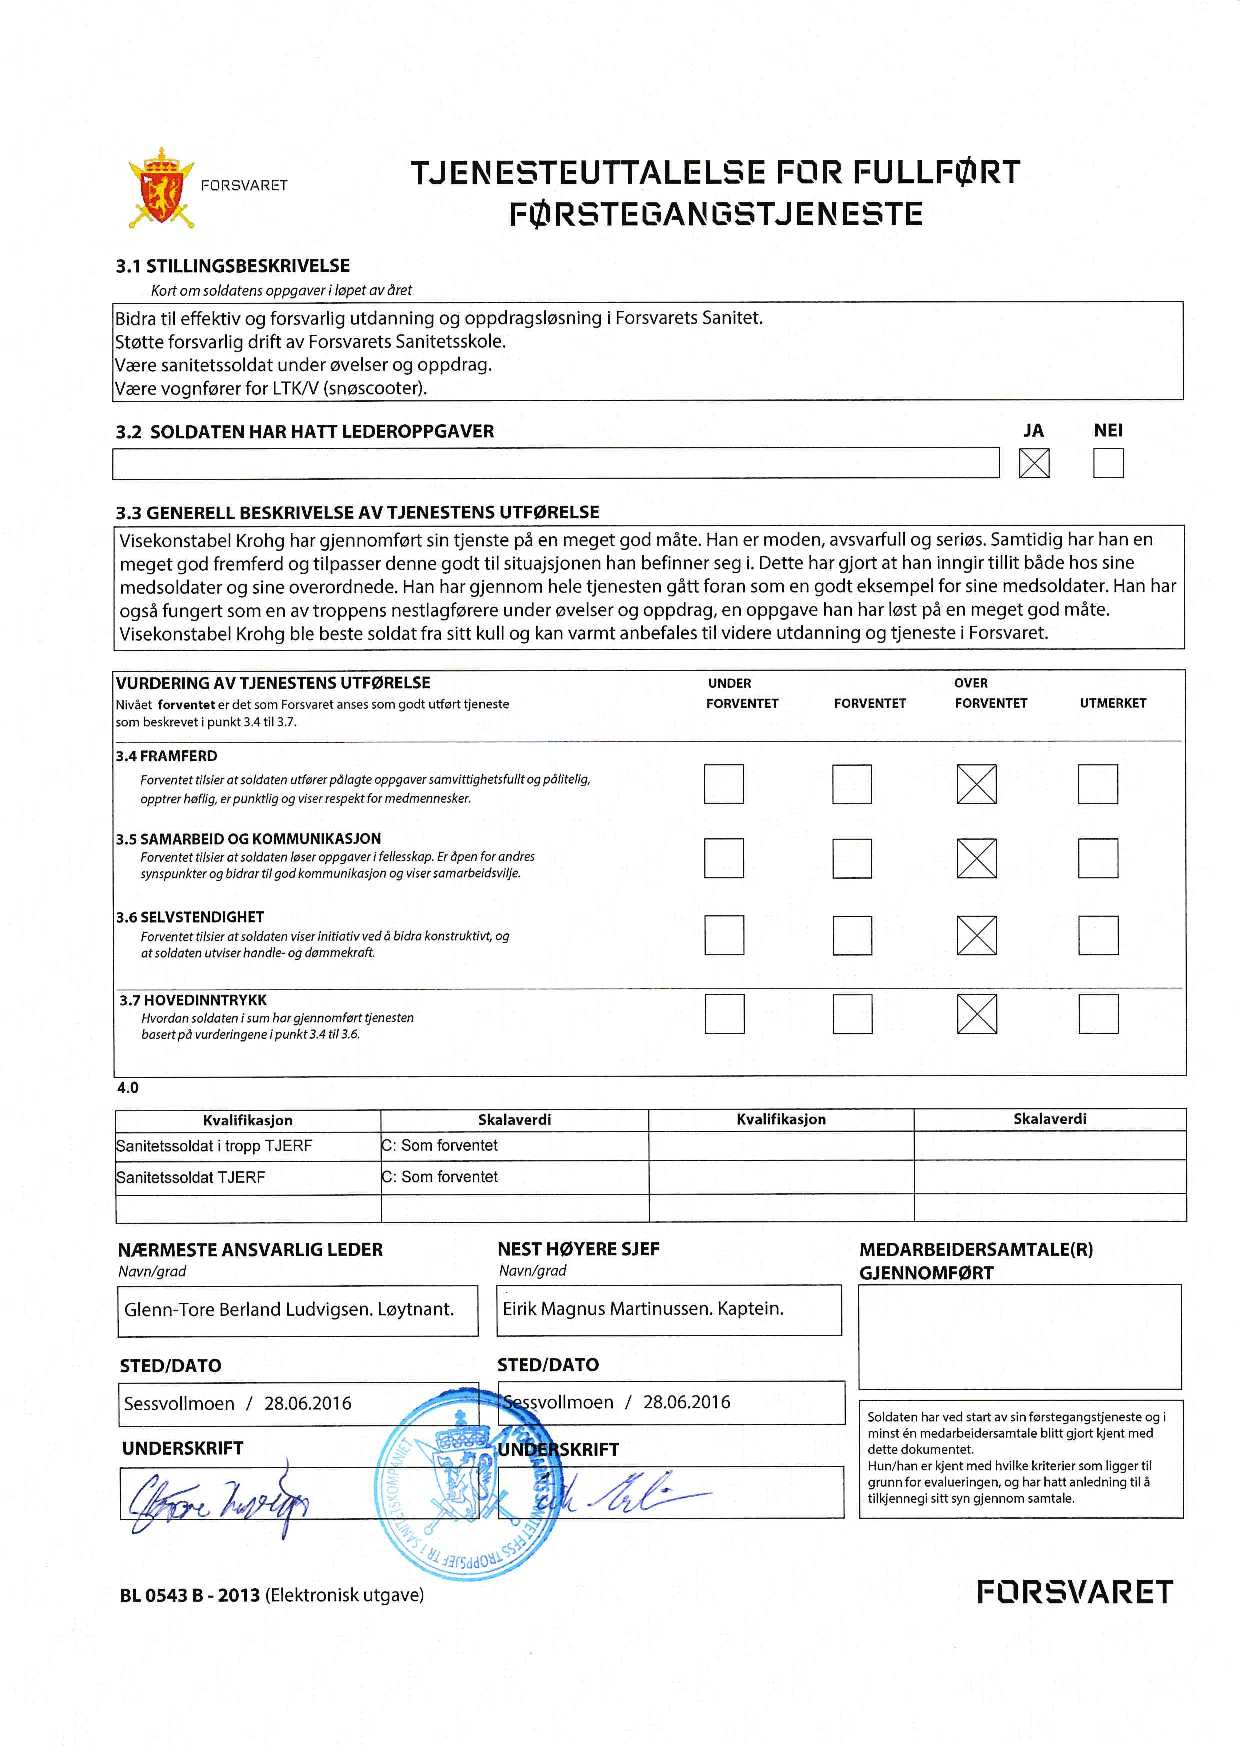
\includepdf[pages=-]{../attester/Tjenesteuttalelse.pdf}

%% \phantomsection
%% \addcontentsline{toc}{subsection}{Portrait}
%% \includepdf[pages=-]{../attester/Attest_Diplom-Is.pdf}

%% \phantomsection
%% \addcontentsline{toc}{subsection}{Portrait}
%% 
\includepdf[pages=-]{../attester/Attest_Telemark_Distribusjon.JPG}

%% \phantomsection
%% \addcontentsline{toc}{subsection}{Portrait}
%% 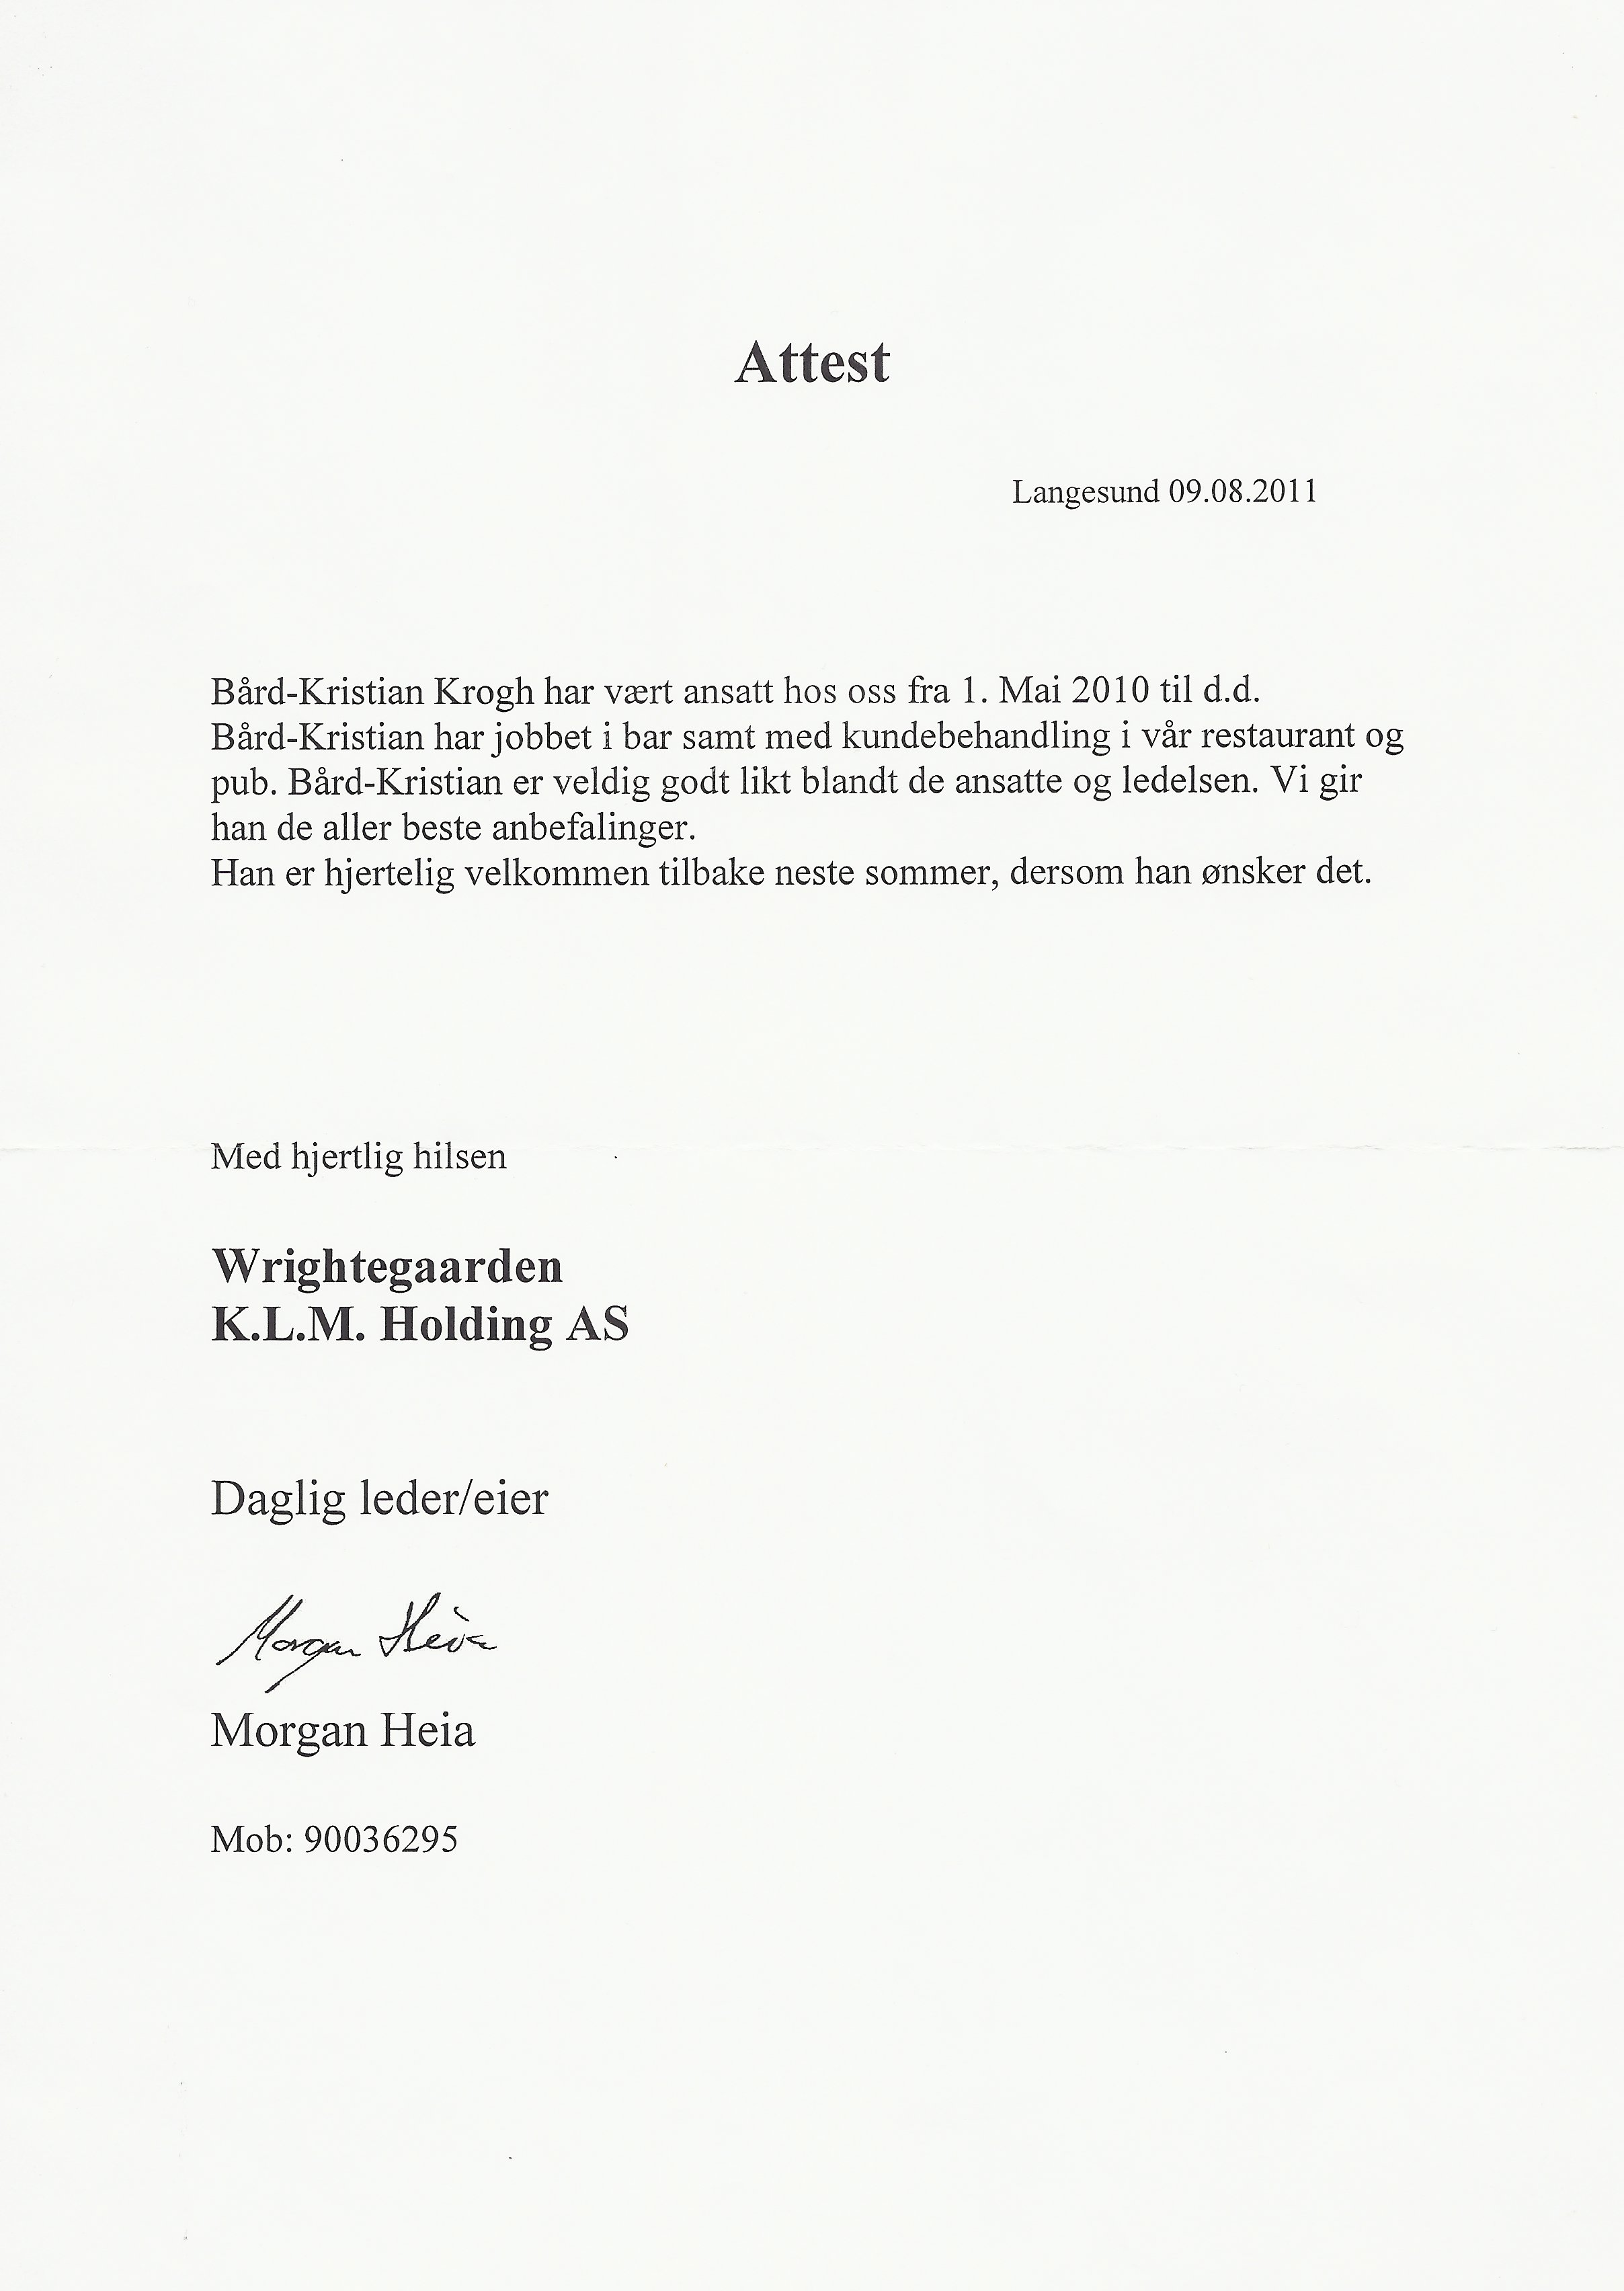
\includepdf[pages=-]{../attester/Attest_Wrightegaarden.JPG}



%-------------------Cover letter------------------------------------------------------------------------

%\input{coverletter.tex}                             % Include cover letter from coverletter.tex

%-------------------Document End------------------------------------------------------------------------

\end{document}

%% end of file `main.tex'.
